\documentclass[12pt]{extarticle}
\usepackage[]{algorithm2e}
\usepackage[utf8]{inputenc}
\usepackage[T1]{fontenc}
\usepackage[french]{babel}
\usepackage{graphicx}
\usepackage{amsmath}
\usepackage{amssymb}
\usepackage{array}
\usepackage{tikz}
\usepackage{url}
\usepackage[hidelinks]{hyperref}

\title{Étude et utilisation des SAT-Solveurs}
\author{Anonyme | Joseph Priou}
\date{Juin 2019}

\newtheorem{mydef}{Définition}
\newtheorem{mytheorem}{Théroème}
\newtheorem{myprop}{Proposition}

\newcolumntype{C}[1]{>{\centering\let\newline\\\arraybackslash\hspace{0pt}}m{#1}}
\SetKwProg{Fn}{Function}{}{}

\begin{document}

\maketitle

\begin{center}
\href{https://github.com/FauconFan/Sat_solver}{https://github.com/FauconFan/Sat\_solver} 
\end{center}

\vspace{2cm}

\section*{Introduction}

Le problème SAT désigne le problème de décision qui, pour une formule logique propositionnelle, détermine s'il existe une distribution de valeurs de vérité qui satisfait la formule.

Il s'agit du premier problème NP-complet donné par le théorème de Cook. Il s'agit d'un problème particulièrement important, car si on arrive à montrer que SAT est soluble en temps polynomial, alors $P = NP$. C'est notamment le 4ème problème du millénaire.

On s'intéresse ici au problème SAT et comment on peut résoudre efficacement une instance de ce problème.

Un SAT-solveur est un programme qui prend une formule logique propositionnelle et détermine s'il existe une telle distribution. Il existe de nombreuses techniques pour essayer de résoudre le problème SAT.

Nous allons également implémenter la modélisation de problèmes à l'aide de formules propositionnelles, comme le problème des N Reines, le Sudoku ou le puzzle des nonogrammes.

\newpage

% \setcounter{tocdepth}{1} % only show sections
\tableofcontents

\newpage

\section{Définitions et propositions essentielles}

\begin{mydef}
Une variable propositionnelle est une variable ayant pour valeur vrai (1) ou faux (0).
\end{mydef}

Soit $P$ l'ensemble des variables propositionnelles.

\begin{mydef} 
L'ensemble des formules propositionnelles est le plus petit ensemble contenant les variables propositionnelles clos par les connecteurs logiques $\lnot$, $\lor$, $\land$ et $\rightarrow$.
\end{mydef}

\begin{mydef}
Une distribution de distribution de valeurs de vérité est une application de $P$ dans $\{ 0, 1\}$
\end{mydef}

\begin{mydef}
Soit $F$ une formule et $\delta : P \rightarrow \{0, 1\}$ une distribution de valeurs de vérité. $\delta$ satisfait $F$ si et seulement si lorqu'on interprète F par $\delta$ F est vraie.
\end{mydef}

\begin{mydef}
Une formule est satisfaisable s'il existe une distribution qui la satisfait. 
\end{mydef}

\begin{mydef}
Un littéral est une variable propositionnelle ou sa négation. On se permettra parfois de désigner l'opposé du littéral l par la négation de ce littéral $\lnot{l}$.
\end{mydef}

\begin{mydef}
Une clause est une disjonction de littéraux. On appelle clause vide une clause qui ne contient pas de littéraux. On appelle aussi clause unitaire une clause qui ne contient qu'un seul littéral.
\end{mydef}

\begin{mydef}
Une formule propositionnelle sous forme normale conjonctive (FNC) est une conjonction de clauses.
\end{mydef}

\begin{mydef}
Soit v une variable. On parle de variable positive quand le littéral $\lnot{v}$ n'est présente dans aucune clause d'une formule FNC ou de variable négative si le littéral v n'est présente dans aucune clause. On dit que le littéral est pur si la variable associée n'est présente que positivement ou si elle n'est présente que négativement.
\end{mydef}

\begin{myprop}
Toute formule propositionnelle est équivalente à une formule sous forme normale conjonctive.
\end{myprop}

\subsection*{Transformation d'une formule en FNC}

\begin{myprop}
Pour toute formule propositionnelle, on peut trouver une formule, en temps polynomial, équisatisfaisable sous forme normale conjonctive.
\end{myprop}

Soient F une formule quelconque et $P_1$ l’ensemble des variables propositionnelles de F. Soient $F = F_1, F_2, ..., F_m, F_{m + 1}, ..., F_t$ les sous-formules de F telles que pour tout $i \in \{1, ..., m\}$, $F_i \not\in P_1$ et pour tout $i \in \{m + 1, ..., t\}$, $F_i \in P_1$.\\
L'algorithme ci-dessous transforme F en une FNC F' équisatisfaisable sur un nouvel ensemble $P_2$ de variables propositionnelles.\\
Pour toute sous-formule $F_i$ de F, on associe une variable propositionnelle $p_i \in P_2$ que l'on interprète par "Si $p_i$ est vraie alors la sous-formule $F_i$ est vraie". On a donc $P_2 = \{p_1, ..., p_t\}$. \\
Pour tout $i \in \{1, ..., m\}$, on définit une formule $\phi_i$ telle que :
\begin{itemize}
    \item si $F_i = \lnot{F_j}$, $\phi_i =  (p_i \leftrightarrow \lnot{p_j})$
    \item si $F_i = F_j \land F_k$, $\phi_i =  (p_i \leftrightarrow p_j \land p_k)$
    \item si $F_i = F_j \lor F_k$, $\phi_i =  (p_i \leftrightarrow p_j \lor p_k)$
\end{itemize}
Pour chacun des cas, $\phi_i$ est équivalente à une conjonction de clause (voir dans l'algorithme ci-après).\\
La formule : $$F' = p_1 \land \bigwedge_{i \in \{1, ..., m\}}\phi_i $$ est équisatisfaisable avec F. \\
On peut remarquer que F' respecte les propriétés suivantes : 
\begin{itemize}
    \item $|P_2| = t$.
    \item F' contient au plus $(3 \times t + 1)$ clauses.
    \item Chaque clause de F' est de longueur au plus 3.
\end{itemize}

\subsubsection*{Algorithme}
\begin{algorithm}[H]
 \Fn{Convert\_to\_fnc (F)}{
 \KwData{Une formule F quelconque}
 \KwResult{Une FNC F' équisatisfaisable avec F}
 F' = $p_1$ \\
 \ForEach{$F_i$ sous-formule de $F$}{
    \Switch{$F_i$}{
        \Case{$F_i = \lnot{F_j}$}{
            $F' \leftarrow F' \land (\lnot{p_i} \lor \lnot{p_j}) \land (p_i \lor p_j)$
        }
        \Case{$F_i = F_j \lor F_k$}{
            $F' \leftarrow F' \land (\lnot{p_i} \lor p_j \lor p_k) \land (\lnot{p_j} \lor p_i) \land (\lnot{p_k} \lor p_i)$
        }
        \Case{$F_i = F_j \land F_k$}{
            $F' \leftarrow F' \land (\lnot{p_i} \lor p_j) \land (\lnot{p_i} \lor p_k) \land (p_i \lor \lnot{p_j} \lor \lnot{p_k})$
        }
    }
 }
 return F'
}
\end{algorithm}
\vspace{2em}

Ainsi le problème SAT se réduit en temps polynomial à trouver si une FNC est satisfaisable.
De plus, toute clause peut être réduit de façon polynomiale à une conjonction de 3-clauses (clauses contenant au plus 3 littéraux). \\

Par la suite, on ne s'intéressera qu'au problème "SAT-FNC".

\newpage
\section{Méthode des coupures}

\subsection{Règle de coupure}

La règle de résolution ou règle de coupure affirme:

$$\frac{p \lor L_1 \lor ... \lor L_n\hspace{2cm}\lnot{p} \lor M_1 \lor ... \lor M_k}{L_1 \lor ... \lor L_n \lor M_1 \lor ... \lor M_k}$$

Ainsi une coupure permet de construire une clause à partir de deux autres clauses s'il existe un littéral présent dans l'une des clauses et son opposé dans l'autre clause.

\subsection{Résolution par coupure}

Une résolution par coupure consiste à répéter l'algorithme suivant :

\begin{itemize}
    \item Enlever toutes les tautologies
    \item Enlever toutes les clauses contenant un littéral pur
    \item Choisir une variable p, puis appliquer la règle de coupure entre toutes les clauses où p est présente et toutes les clauses où $\lnot{p}$ est présente.
\end{itemize}

Remarquons que, à chaque étape, il y a au moins une variable qui disparaît. Deux cas se présentent, ou bien on obtient la clause vide et la formule n'est pas satisfaisable, ou bien on arrive jusqu'à l'épuisement des clauses, alors la formule est satisfaisable.

Comme il y a un nombre fini de variables, cette résolution se termine car, à chaque étape, on retire toutes les occurences d'au moins une variable.

\newpage
\section{Théorème de Haken}

\subsection{PHP}

Le Pigeon Hole Principle ou $PHP_n^{n + 1}$, affirme que si n + 1 pigeons doivent aller dans n nids, alors il y a au moins un nid qui habrite 2 pigeons. Ainsi le problème qui consiste à mettre n + 1 pigeons dans n nids sachant que chaque nid ne peut contenir qu'un seul pigeon est insoluble.

\vspace{2em}

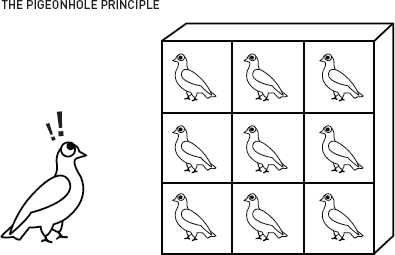
\includegraphics[]{pigeonhole-principle1.png}

\vspace{2em}

On souhaite montrer comment on peut représenter le problème du $PHP_n^{n + 1}$ à l'aide d'une formule sous forme normale conjonctive. On suppose que n est un entier natuel non nul.

Pour tout $1 \leq i \leq n + 1$, et $1 \leq j \leq n$, on considère $x_i^j$ variable propositionnelle et on conviendra qu'elle est vraie si le i-ième pigeon est dans le j-ième nid.

Nous avons deux contraintes à représenter : celle que chaque pigeon doit être présent dans au moins un nid, et que chaque nid ne peut accueillir plus d'un pigeon.

Pour la première contrainte, soit $\phi_i$ la clause qui correspond au fait qu'un pigeon doit se trouver dans au moins un nid.

$$ \phi_i = \bigvee_{1 \leq j \leq n} x_i^j $$

Pour la seconde contrainte, soit $\psi_j$ la conjonction de clauses qui correspond au fait qu'un nid ne peut accueillir deux pigeons.

$$ \psi_j = \bigwedge_{1 \leq j \leq n + 1} \Big( \underset{r \neq s}{\bigwedge_{1 \leq r, s \leq n}} \big( \lnot{x_r^j} \lor \lnot{x_s^j} \big) \Big) $$

Ainsi on peut représenter le problème $PHP_n^{n + 1}$ par la formule FNC suivante:

$$\Big( \bigwedge_{1 \leq i \leq n + 1} \phi_i \Big) \land \Big( \bigwedge_{1 \leq j \leq n} \psi_j \Big)$$

\subsection{Théorème de Haken}

On appelle preuve par réfutation d'une formule F en forme normale conjonctive toute suite de clauses $(C_1, C_2, ..., C_t)$ où $C_t$ est la clause vide et les clauses $C_i$ sont des clauses soit issues de F, soit le résultat d'une coupure entre 2 clauses $C_j$ et $C_k$ avec $j \neq k$, $j, k < i$. On note aussi que t désigne la longueur de la preuve.

\begin{mytheorem}
Le théorème de Haken affirme que, pour n assez grand, toute preuve par réfutation du $PHP_n^{n + 1}$ est de longueur au moins égale à $2^{\Omega(n)}$ avec $\Omega$ une fonction linéaire (non nulle).
\end{mytheorem}

Le théorème de Haken nous montre qu'il existe des exemples (ici PHP) qui ne peuvent être résolus en temps polynomial, avec la méthode de coupures. Donc la méthode des coupures n'est pas un algorithme qui donne une réponse polynomiale pour le problème SAT.

On s'intéresse maintenant à des algorithmes performants qui sont envisagés dans de vrais SAT-solveurs.


\section{L'algorithme DPLL}

DPLL (ou Davis–Putnam–Logemann–Loveland) est un algorithme de backtracking (ou de retour sur trace) qui permet de résoudre le problème SAT en un temps acceptable dans beaucoup de cas.

On rappelle qu'un algorithme de backtracking est un algorithme où l'on veut tester toutes les possibilités récursivement afin de trouver une solution. On va donc envisager de nombreux cas qui vont être faux, on va donc revenir sur nos choix, faire un retour sur trace (backtrack) afin d'envisager de nouveaux cas. On utilise ce genre d'algorithmes pour des problèmes de décision ou d'optimisation.

DPLL se distingue d'un simple algorithme de backtracking car il essaie de déduire des assignations par rapport aux clauses qui lui reste.

\subsection{Algorithme}

La présence d'une clause unitaire entraîne une propagation unitaire du littéral présent dans la clause unitaire. On appelle l ce littéral et on désigne par $\lnot{l}$ la négation de ce littéral.

La propagation unitaire propage l sur le reste des clauses. Si l est présente dans la clause, alors la clause est satisfaite. Si $\lnot{l}$ est présente dans la clause, on peut simplifier la clause en supprimant la présence de $\lnot{l}$ dans la clause. La propagation unitaire peut entraîner de nouvelles clauses unitaires. C'est ce que fait la fonction 'propagation-unitaire()' dans l'algorithme.

De même, si un littéral est pur, on peut alors faire une assignation sur la variable associé à ce littéral en satisfaisant toutes les clauses qui contiennent ce littéral. Cette action peut entraîner que d'autres littéraux deviennent purs. La fonction 'affecter-litteral-pur()' va juste détecter si le littéral est positif ou négatif et satisfaire toutes les clauses concernées.

L'algorithme DPLL contient une heuristique qui correspond au choix de la variable que l'on va assigner lorsqu'on ne sait pas quoi déduire. Il s'agit de la fonction 'choisir-litteral()' dans l'algorithme. Ce choix peut dépendre du nombre d'occurrences de la variable ou encore de la présence de cette variable dans de grosses clauses par exemple.

On définit la fonction DPLL qui retourne SAT si la formule est satisfaisable et UNSAT sinon :

\vspace{2em}

\begin{algorithm}[H]
 \Fn{DPLL (F)}{
 \KwData{Une formule F}
 \KwResult{F est-elle satisfaisable ?}
 \While{F contient une clause unitaire C}{F $\leftarrow$ propagation-unitaire(F, C)}
 \lIf{F contient la clause vide}{return \textbf{UNSAT}}
 \While{F contient un littéral pur l}{F $\leftarrow$ affecter-litteral-pur(F, l)}
 \lIf{F ne contient que des clauses satisfaites}{return \textbf{SAT}}
 l $\rightarrow$ choisir-litteral(F) \\
 return (DPLL(F $\land \{l\}$) ou  DPLL(F $\land \{\lnot{l}\}$)
}
\end{algorithm}

\subsection{Exemple}

Prenons un exemple où nous détaillons l'exécution de l'algorithme DPLL.

$F = C_1 \land C_2 \land C_3 \land C_4 \land C_5 \land C_6 \land C_7$ \\
$C_1 = (x_1 \lor x_2 \lor \lnot{x_4})$ \\
$C_2 = (\lnot{x_1} \lor x_3 \lor \lnot{x_4})$ \\
$C_3 = (x_1 \lor x_3 \lor x_4)$ \\
$C_4 = (\lnot{x_1} \lor \lnot{x_3} \lor \lnot{x_4})$ \\
$C_5 = (\lnot{x_1} \lor x_2 \lor x_4)$ \\
$C_6 = (x_1 \lor x_3 \lor \lnot{x_4})$ \\
$C_7 = (x_3 \lor \lnot{x_4})$ \\

Initialisation:

$\delta = \{\}$

1er tour:

F ne contient pas de clauses cohérentes ni la clause vide. F ne contient pas non plus de clauses unitaires. Or $x_2$ n'est présente que positivement, on peut alors supprimer les clause 1 et 5:

$F = C_2 \land C_3 \land C_4 \land C_6 \land C_7$ \\
$C_2 = (\lnot{x_1} \lor x_3 \lor \lnot{x_4})$ \\
$C_3 = (x_1 \lor x_3 \lor x_4)$ \\
$C_4 = (\lnot{x_1} \lor \lnot{x_3} \lor \lnot{x_4})$ \\
$C_6 = (x_1 \lor x_3 \lor \lnot{x_4})$ \\
$C_7 = (x_3 \lor \lnot{x_4})$ \\

$\delta = \{(x_2, Vrai)\}$

On prend la variable $x_4$ et on rajoute la clause unitaire $(x_4)$.

$F = C_2 \land C_3 \land C_4 \land C_6 \land C_7 \land C_8$ \\
$C_2 = (\lnot{x_1} \lor x_3 \lor \lnot{x_4})$ \\
$C_3 = (x_1 \lor x_3 \lor x_4)$ \\
$C_4 = (\lnot{x_1} \lor \lnot{x_3} \lor \lnot{x_4})$ \\
$C_6 = (x_1 \lor x_3 \lor \lnot{x_4})$ \\
$C_7 = (x_3 \lor \lnot{x_4})$ \\
$C_8 = (x_4)$

$\delta = \{(x_2, Vrai)\}$

2ème tour:

F ne contient pas de clauses cohérentes ni la clause vide. F contient une clause unitaire $C = (x_4)$. Ainsi on fait de la propagation unitaire.

$F = C_2 \land C_4 \land C_6 \land C_7$ \\
$C_2 = (\lnot{x_1} \lor x_3)$ \\
$C_4 = (\lnot{x_1} \lor \lnot{x_3})$ \\
$C_6 = (x_1 \lor x_3)$ \\
$C_7 = (x_3)$ \\

$\delta = \{(x_2, Vrai), (x_4, Vrai)\}$

La 7ème clause devient alors unitaire et on peut la propager.

$F = C_4$ \\
$C_4 = (\lnot{x_1})$ \\

$\delta = \{(x_2, Vrai), (x_3, Vrai), (x_4, Vrai)\}$

De même avec la 4ème Clause.

$F = \emptyset$

$\delta = \{(x_1, Faux), (x_2, Vrai), (x_3, Vrai), (x_4, Vrai)\}$

\newpage
\section{L'algorithme CDCL}

Basé sur DPLL, CDCL (ou Conflict-Driven Clause Learning) est un algorithme qui peut apprendre de nouvelles clauses lorsque celui-ci rencontre des conflits.

Il fait également un backtracking non chronologique, c'est à dire un backtracking d'une ou plusieurs étapes, permettant de réduire le nombre de conflits en interprétant au maximum les clauses apprises.

\subsection{Algorithme}

\begin{algorithm}[H]
 \Fn{CDCL (F)}{
 \KwData{Une formule F}
 \KwResult{F est-elle satisfaisable ?}
 decision\_level $\leftarrow 0$ \\
 \While {F contient au moins une clause non satisfaite}{
    \If{propagation unitaire == Conflit}{
        \lIf {decision\_level == 0}{return \textbf{UNSAT}}
         decision\_level $\leftarrow$ conflict\_analysis(F) \\
         backjump (decision\_level) \\
         continue
    }
    \lIf{F ne contient que des clauses satisfaites}{break}
    decision\_level ++ \\
    assign\_value()
    }
 }
 return (\textbf{SAT})
\end{algorithm}

\vspace{2em}

L'algorithme CDCL permet de résoudre des problème en apprenant des clauses à chaque conflit (on rajoute de nouvelles clauses dans la formule).

Il est alors nécessaire de tenir à jour un graphe des implications.
Il s'agit d'un graphe orienté acyclique dont les sommets représentent l'assignation d'une valeur à une variable et les arrêtes modélisent les raisons menant à l'assignation d'une variable.
Ainsi, lorsqu'il y a un conflit, on peut construire une nouvelle clause qui empêchera d'arriver au même conflit en se servant de ce graphe.

Tout comme DPLL, lorsqu'il n'y a plus aucun moyen de déduire des valeurs pour les variables non assignées à partir des variables déjà assignées, l'algorithme décide d'une valeur pour une variable non assignée et calcule les conséquences.

On appelle niveau de décision d'une variable $x$ le nombre de décisions prises par l'algorithme au moment d'assigner une valeur à $x$. Ainsi, au début de l'algorithme, le niveau de décision est 0 et avant chaque assignation par décision, on incrémente le niveau de décision d'un.

Lors d'une propagation unitaire, la déduction d'une valeur pour une variable $x$ d'une clause $C = (x_1, ..., x_n, x)$, se modélise dans le graphe des implications par des arrêtes partant de $x_i$ pour tout $i \in \{1, ..., n\}$ à destination de $x$.

Ainsi, il n'y a jamais d'arrêtes dont la destination est une variable assignée par décision de l'algorithme.

\subsection{Exemple}

Prenons un exemple où nous détaillons l'exécution de l'algorithme CDCL. Dans le graphe des implications, on notera $x = v @ d$ le fait que l'assignation de la valeur $v$ à $x$ a été faite au niveau de décision $d$. \\

$F = C_1 \land C_2 \land C_3 \land C_4 \land C_5 \land C_6 \land C_7 \land C_8$\\
$C_1 = (\lnot{x_1} \lor x_4 \lor x_5)$ \\
$C_2 = (x_4 \lor x_6)$ \\
$C_3 = (\lnot{x_5} \lor \lnot{x_6} \lor \lnot{x_7})$ \\
$C_4 = (x_7 \lor \lnot{x_8})$ \\
$C_5 = (x_2 \lor x_7 \lor x_9)$ \\
$C_6 = (x_8 \lor \lnot{x_9})$ \\
$C_7 = (x_3 \lor x_9 \lor \lnot{x_{10}})$ \\
$C_8 = (x_1 \lor \lnot{x_3} \lor \lnot{x_4} \lor \lnot{x_9} \lor x_{10})$ \\

\noindent Initialisation : Le graphe des implications est vide  \\

\noindent Première décision : $x_1 = 1$ \\
La propagation unitaire ne permet pas de déduire quelque chose. Le graphe des implications est donc réduit à un unique noeud : \\

\begin{tikzpicture}
  [scale=.8]
  \node (n1) at (1,3) {$x_1 = 1 @ 1$};
\end{tikzpicture}

Deuxième décision : $x_2 = 0$ \\
A nouveau, aucune déduction n'est possible avec la propagation unitaire. 
Le graphe devient : \\

\begin{tikzpicture}
  [scale=.8]
  \node (n1) at (1, 2) {$x_1 = 1 @ 1$};
  \node (n2) at (1, 1) {$x_2 = 0 @ 2$};
\end{tikzpicture} \\
Troisième décision : $x_3 = 0$ \\
Le graphe devient : \\

\begin{tikzpicture}
  [scale=.8]
  \node (n1) at (1, 2) {$x_1 = 1 @ 1$};
  \node (n2) at (4, 1) {$x_2 = 0 @ 2$};
  \node (n3) at (1, 1) {$x_3 = 0 @ 3$};
\end{tikzpicture} \\
Quatrième décision : $x_4 = 0$ \\
Par la propagation unitaire, on peut déduire  :
\begin{itemize}
    \item $x_5 = 1$ par $C_1$
    \item $x_6 = 1$ par $C_2$
    \item $x_7 = 0$ par $C_3$
    \item $x_8 = 0$ par $C_4$
    \item $x_9 = 1$ par $C_5$
    \item $x_9 = 0$ par $C_6$
\end{itemize}
Le graphe, avec toutes ces implications, devient : \\

\begin{tikzpicture}
  [scale=.8]
  \node (n1) at (1, 5) {$x_1 = 1 @ 1$};
  \node (n2) at (7, 1) {$x_2 = 0 @ 2$};
  \node (n3) at (1, 1) {$x_3 = 0 @ 3$};
  \node (n4) at (1, 3) {$x_4 = 0 @ 4$};
  \node (n5) at (4, 4) {$x_5 = 1 @ 4$};
  \node (n6) at (4, 2) {$x_6 = 1 @ 4$};
  \node (n7) at (7, 3) {$x_7 = 0 @ 4$};
  \node (n8) at (10, 4) {$x_8 = 0 @ 4$};
  \node (n9) at (13, 3) {$x_9 = 0 @ 4$};
  \node (nk) at (10, 2) {$x_9 = 1 @ 4$};

  \foreach \from/\to in {n4/n5,n1/n5,n4/n6,n5/n7,n6/n7,n7/n8,n7/nk,n2/nk,n8/n9}
  \draw[->] (\from) -- (\to);
  \draw[red, <->] (n9) -- (nk);
\end{tikzpicture} \\

On voit clairement sur ce graphe qu'il y a un conflit (modélisé par la double flèche rouge).
On fait alors une coupe dans le graphe pour dissocier le conflit du reste. \\

\begin{tikzpicture}
  [scale=.8]
  \node (n1) at (1, 5) {$x_1 = 1 @ 1$};
  \node (n2) at (7, 1) {$x_2 = 0 @ 2$};
  \node (n3) at (1, 1) {$x_3 = 0 @ 3$};
  \node (n4) at (1, 3) {$x_4 = 0 @ 4$};
  \node (n5) at (4, 4) {$x_5 = 1 @ 4$};
  \node (n6) at (4, 2) {$x_6 = 1 @ 4$};
  \node (n7) at (7, 3) {$x_7 = 0 @ 4$};
  \node (n8) at (10, 4) {$x_8 = 0 @ 4$};
  \node (n9) at (13, 3) {$x_9 = 0 @ 4$};
  \node (nk) at (10, 2) {$x_9 = 1 @ 4$};

  \foreach \from/\to in {n4/n5,n1/n5,n4/n6,n5/n7,n6/n7,n7/n8,n7/nk,n2/nk,n8/n9}
  \draw[->] (\from) -- (\to);
  \draw[red, <->] (n9) -- (nk);
  \draw (13, 4) -- (14, 4);
  \draw (7, 2) -- (13, 4);
  \draw (7, 2) -- (10, 1);
  \draw (10, 1) -- (12, 1);
\end{tikzpicture} \\

Toutes les variables dont les implications traversent la coupure sont directement responsable du conflit.

Ainsi, les variables $x_2$, $x_7$ et $x_8$ sont impliquées.

Sur le graphe, on peut également voir que $\lnot{x_7} \rightarrow \lnot{x_8}$ donc seules les variables $x_2$ et $x_7$ sont vraiment responsables du conflit. \\

\begin{tikzpicture}
  [scale=.8]
  \node (n1) at (1, 5) {$x_1 = 1 @ 1$};
  \node (n2) at (7, 1) {$x_2 = 0 @ 2$};
  \node (n3) at (1, 1) {$x_3 = 0 @ 3$};
  \node (n4) at (1, 3) {$x_4 = 0 @ 4$};
  \node (n5) at (4, 4) {$x_5 = 1 @ 4$};
  \node (n6) at (4, 2) {$x_6 = 1 @ 4$};
  \node (n7) at (7, 3) {$x_7 = 0 @ 4$};
  \node (n8) at (10, 4) {$x_8 = 0 @ 4$};
  \node (n9) at (13, 3) {$x_9 = 0 @ 4$};
  \node (nk) at (10, 2) {$x_9 = 1 @ 4$};

  \foreach \from/\to in {n4/n5,n1/n5,n4/n6,n5/n7,n6/n7,n7/n8,n7/nk,n2/nk,n8/n9}
  \draw[->] (\from) -- (\to);
  \draw[red, <->] (n9) -- (nk);
  \draw (7, 4) -- (10, 5);
  \draw (10, 3) -- (7, 4);
  \draw (7, 2) -- (10, 3);
  \draw (7, 2) -- (10, 1);
\end{tikzpicture} \\

On a alors $(\lnot{x_2} \land \lnot{x_7}) \rightarrow$ "conflit" donc "non conflit" $\rightarrow (x_2 \lor x_7)$. On peut donc apprendre la clause $C_9 = (x_2 \lor x_7)$ car la formule $F_1 = F \land C_9$ est équisatisfaisable avec $F$. \\

On note ici que nous avons décidé de s'arrêter à $x_7 = 0$, mais nous aurions pu revenir encore plus loin dans le graphe des implications et prendre alors une autre clause. Nous allons expliquer plus loin notre choix, mais nous décidons de nous arrêter au point d'articulation le plus proche de notre conflit. Il se trouve que, dans cet exemple, ce point est le point $x_7 = 0$. \\

Il faut maintenant revenir à un niveau de décision inférieur afin de prendre en compte la nouvelle clause et de ne pas retomber dans le même conflit.

Pour calculer le niveau de décision auquel on doit revenir, on regarde le niveau de décision des variables impliquées dans la nouvelle clause et on prend le maximum sans compter le niveau de décision actuel.
On revient donc au niveau 2 et grâce à la nouvelle clause, on peut déduire par propagation unitaire que $x_7 = 1$.

Le graphe devient alors le suivant : \\

\begin{tikzpicture}
  [scale=.8]
  \node (n1) at (1, 2) {$x_1 = 1 @ 1$};
  \node (n2) at (4, 2) {$x_2 = 0 @ 2$};
  \node (n7) at (7, 1) {$x_7 = 1 @ 2$};

  \foreach \from/\to in {n2/n7}
  \draw[->] (\from) -- (\to);
\end{tikzpicture} \\
Troisième décision : $x_4 = 0$ \\
Par la propagation unitaire, on peut déduire  :
\begin{itemize}
    \item $x_5 = 1$ par $C_1$
    \item $x_6 = 1$ par $C_2$
    \item $x_7 = 0$ par $C_3$
\end{itemize}
Le graphe avec toutes ces implications devient : \\

\begin{tikzpicture}
  [scale=.8]
  \node (n1) at (1, 4) {$x_1 = 1 @ 1$};
  \node (n2) at (7, 4) {$x_2 = 0 @ 2$};
  \node (n7) at (10, 3) {$x_7 = 1 @ 2$};
  \node (n4) at (1, 2) {$x_4 = 0 @ 3$};
  \node (n5) at (4, 3) {$x_5 = 1 @ 3$};
  \node (n6) at (4, 1) {$x_6 = 1 @ 3$};
  \node (nk) at (7, 2) {$x_7 = 0 @ 3$};

  \foreach \from/\to in {n2/n7,n4/n5,n1/n5,n4/n6,n5/nk,n6/nk}
  \draw[->] (\from) -- (\to);
  \draw[red, <->] (n7) -- (nk);
\end{tikzpicture} \\

On a de nouveau un conflit donc on effectue, sur le graphe, une coupure pour séparer le conflit du reste. \\

\begin{tikzpicture}
  [scale=.8]
  \node (n1) at (1, 4) {$x_1 = 1 @ 1$};
  \node (n2) at (7, 4) {$x_2 = 0 @ 2$};
  \node (n7) at (10, 3) {$x_7 = 1 @ 2$};
  \node (n4) at (1, 2) {$x_4 = 0 @ 3$};
  \node (n5) at (4, 3) {$x_5 = 1 @ 3$};
  \node (n6) at (4, 1) {$x_6 = 1 @ 3$};
  \node (nk) at (7, 2) {$x_7 = 0 @ 3$};

  \foreach \from/\to in {n2/n7,n4/n5,n1/n5,n4/n6,n5/nk,n6/nk}
  \draw[->] (\from) -- (\to);
  \draw[red, <->] (n7) -- (nk);
  \draw (4, 2) -- (10, 4);
  \draw (4, 2) -- (7, 1);
  
\end{tikzpicture} \\

Les variables directement responsables du conflit sont alors $x_2$, $x_5$ et $x_6$.
Mais $\lnot{x_4} \rightarrow x_6$ et $x_1 \land \lnot{x_4} \rightarrow x_5$ donc les variables vraiment responsables du conflit sont $x_1$, $x_2$ et $x_4$ donc on peut apprendre la clause $C_{10} = (\lnot{x_1} \lor x_2 \lor x_4)$.
On revient ensuite au niveau de décision 2 et on peut déduire, grâce à la nouvelle clause que $x_4 = 1$. \\
On obtient alors le graphe suivant : \\

\begin{tikzpicture}
  [scale=.8]
  \node (n1) at (1, 4) {$x_1 = 1 @ 1$};
  \node (n2) at (1, 2) {$x_2 = 0 @ 2$};
  \node (n7) at (4, 1) {$x_7 = 1 @ 2$};
  \node (n4) at (4, 3) {$x_4 = 1 @ 2$};

  \foreach \from/\to in {n2/n7,n1/n4,n2/n4}
  \draw[->] (\from) -- (\to);
  
\end{tikzpicture} \\
Troisième décision : $x_3 = 0$ \\
On ne peut rien en déduire. \\

\begin{tikzpicture}
  [scale=.8]
  \node (n1) at (1, 4) {$x_1 = 1 @ 1$};
  \node (n2) at (1, 2) {$x_2 = 0 @ 2$};
  \node (n7) at (4, 1) {$x_7 = 1 @ 2$};
  \node (n4) at (4, 3) {$x_4 = 1 @ 2$};
  \node (n3) at (7, 4) {$x_3 = 0 @ 3$};

  \foreach \from/\to in {n2/n7,n1/n4,n2/n4}
  \draw[->] (\from) -- (\to);
  
\end{tikzpicture} \\
Quatrième décision : $x_5 = 1$ \\
Par propagation, on en déduit : 
\begin{itemize}
    \item $x_6 = 1$ par $C_3$
\end{itemize}
On obtient le graphe suivant : \\

\begin{tikzpicture}
  [scale=.8]
  \node (n1) at (1, 4) {$x_1 = 1 @ 1$};
  \node (n2) at (1, 2) {$x_2 = 0 @ 2$};
  \node (n7) at (4, 1) {$x_7 = 1 @ 2$};
  \node (n4) at (4, 3) {$x_4 = 1 @ 2$};
  \node (n3) at (7, 4) {$x_3 = 0 @ 3$};
  \node (n5) at (10, 1) {$x_5 = 1 @ 4$};
  \node (n6) at (7, 2) {$x_6 = 0 @ 4$};

  \foreach \from/\to in {n2/n7,n1/n4,n2/n4,n5/n6,n7/n6}
  \draw[->] (\from) -- (\to);
  
\end{tikzpicture} \\
Cinquième décision : $x_9 = 0$ \\
Par propagation, on en déduit : 
\begin{itemize}
    \item $x_{10} = 0$ par $C_7$
\end{itemize}
On obtient le graphe suivant : \\

\begin{tikzpicture}
  [scale=.8]
  \node (n1) at (1, 4) {$x_1 = 1 @ 1$};
  \node (n2) at (1, 2) {$x_2 = 0 @ 2$};
  \node (n7) at (4, 1) {$x_7 = 1 @ 2$};
  \node (n4) at (4, 3) {$x_4 = 1 @ 2$};
  \node (n3) at (7, 4) {$x_3 = 0 @ 3$};
  \node (n5) at (10, 1) {$x_5 = 1 @ 4$};
  \node (n6) at (7, 2) {$x_6 = 0 @ 4$};
  \node (n9) at (13, 4) {$x_9 = 0 @ 5$};
  \node (n10) at (10, 3) {$x_{10} = 0 @ 5$};

  \foreach \from/\to in {n2/n7,n1/n4,n2/n4,n5/n6,n7/n6,n3/n10,n9/n10}
  \draw[->] (\from) -- (\to);
  
\end{tikzpicture} \\

Toutes les clauses sont satisfaites (Peu importe la valeur de $x_8$) donc $F$ est satisfaisable.

\subsection{Bounded learning}

L'apprentissage non maitrisé de nouvelles clauses peut cependant diminuer l'efficacité de l'algorithme. En effet, lorsqu'il y a beaucoup de conflits (notamment quand une formule est longue), on ajoute beaucoup de nouvelles clauses à la formule et celle-ci peut devenir tellement longue que la moindre opération dessus s'avère très coûteuse en temps. \\
Deux stratégies sont alors possibles pour limiter l'apprentissage excessif de clauses (qui peuvent être combinées) :
\begin{itemize}
    \item La première consiste à sélectionner les clauses que l'on apprend à l'aide d'un critère sur la longueur de la clause, c'est à dire que l'on apprend seulement les clauses de longueur i ou moins (i fixé).
    \item La deuxième est appelée la "i-relevance". Elle consiste à oublier des clauses que l'on a apprises (on ne supprime pas de clauses de la formule originale) selon le nombre de littéraux non assignés. Ainsi, à un moment donné, on regarde les clauses apprises et si certaines d'entre elles contiennent plus de i littéraux non assignés, on les supprime.
\end{itemize}

\subsection{Restart}

Il se peut que durant une exécution de l'algorithme, on se retrouve dans une zone de l'arbre de décision où il y a de nombreux conflits et où les clauses apprises sont peu utiles.  
Ainsi, une autre optimisation possible, appelée restart, consiste à oublier tous les choix ainsi que les assignements qui en découlent, lorsqu'un certain nombre de conflits à été atteint. 
On recommence ainsi une exécution dans une nouvelle zone où les clauses apprises augmentent les chances de ne pas retomber dans le même espace que précédemment.

\subsection{Heuristiques}

Contrairement à DPLL, CDLC a de nombreuses heuristiques possibles et à plusieurs niveaux. \\

La première heuristique consiste à choisir les clauses que l'on veut apprendre lors d'un conflit. Dans l'exemple que nous avons pris, nous apprenons la clause qui ne contient qu'un seul littéral dans le niveau de décision courant. Ce littéral correspond à un point d'articulation dans le chemin du choix initial du niveau de décision courant vers le conflit.

Il arrive souvent qu'il y ait plusieurs points d'articulation, dans notre exemple nous avons choisi le point d'articulation le plus proche du conflit. Ce choix correspond au 1-UIP appelé "first uniq implication point"%, ce qui correspond au premier point d'articulation
. Un autre choix possible est celui du Last-UIP 
%correpond au Last-UIP, 
qui prend le dernier point d'articulation dans le graphe à savoir le choix du niveau de décision courant. Dans notre exemple, il s'agit du point $x_4 = 0$.

On pourrait également apprendre plusieurs clauses, autant de clauses que nous permet le graphe des implications en remontant la propagation unitaire. Néanmoins, on remarque qu'en pratique, seules les clauses qui ne contiennent qu'un seul littéral dans le niveau de décision courant sont gardées. On fait ce choix là car la clause est alors plus pertinente car elle ne contient pas de redondance d'information, par exemple, lorsque l'on a considéré lors du premier conflit la clause avec les variables $x_2$, $x_7$ et $x_8$. On peut dire aussi que l'on fait ce choix, car lorsqu'on revient à un niveau de décision antérieur par backtracking non chronologique, la clause que l'on vient de rajouter devient unitaire et on peut alors se retrouver dans un état jamais exploré auparavant dans le graphe des implications. \\

Pour l'apprentissage de clauses, le choix de la taille des clauses que l'on apprend est une heuristique. Si ce nombre est trop haut, on peut apprendre beaucoup trop de clauses, si ce nombre est trop bas, on pourrait ne pas apprendre des clauses utiles dans l'espace de recherche dans lequel on est. \\

D'autres heuristiques existent pour la gestion de l'oubli des clauses afin d'éviter de se retrouver avec un grand nombre de clauses. Comme nous l'avons souligné, la i-relevance permet d'oublier les clauses dont au moins i littéraux ne sont pas assignés au moment l'assignement courant. Le choix de ce i est alors une heuristique.

De plus, dans notre implémentation, nous avons décidé d'avoir un seuil qui correspond au double du nombre de clauses de la formule initiale. Ce seuil détermine le moment où l'on utilise la i-relevance pour oublier les clauses qui sont le moins pertinentes à ce moment.
Cependant, on peut apprendre des clauses que l'on souhaite ne jamais oublier, c'est à dire celles contenant moins de i littéraux. On augmentera alors ce seuil lorsque l'on apprend de telles clauses. \\

D'autre part, on doit choisir quand est-ce que l'on décide de faire un restart. On peut, par exemple, définir un nombre de conflit maximum qui, lorsqu'on l'atteint, provoque le restart de l'algorithme. Il faut également choisir le taux multiplicatif pour concerver la complétude. \\

Tous ces choix montrent que CDCL est vraiment différent d'une implémentation à une autre. Ce sont tous ces choix qui, en faisant des benchmarks et des analyses, permettent d'avoir des SAT-solveurs vraiment efficaces.

\newpage
\section{Comparaison DPLL / CDCL}

\subsection{Pigeon Hole Principle}

\begin{table}[h!]
\centering
\begin{tabular}{|l||C{2cm}|C{2cm}|C{2cm}|C{2cm}|C{2cm}|}
    \hline & DPLL & \multicolumn{4}{|c|}{CDCL}\\
    \hline & & & BL & R & BL R\\
    \hline PHP 5 & 0.00s & 0.01s & 0.02s & 0.02s & 0.03s \\
    \hline PHP 6 & 0.01s & 0.05s & 0.05s & 0.05s & 0.05s \\
    \hline PHP 7 & 0.06s & 0.27s & 0.16s & 0.24s & 0.16s \\
    \hline PHP 8 & 0.44s & 2.09s & 1.55s & 1.68s & 7.92s \\
    \hline PHP 9 & 4.20s & 18.78s & 14.58s & 20.89s & 81.26s \\
    \hline PHP 10 & 46.08s & 193.48s & 187.71s & 298.63s & 1084.60s \\
    \hline
\end{tabular}
\caption{Tableau de comparaison du temps d'exécution pour PHP}
\end{table}

Ce premier tableau nous montre que DPLL est plus efficace que CDCL, quelque soit les améliorations apportées à ce dernier, sur le probème $PHP_n^{n+1}$ et que la différence s'accentue quand n augmente. Cette différence de performance peut s'expliquer par le fait que les clauses que l'on apprend lors des conflits sont majoritairement des clauses très longues et donc très peu utilisable pour éviter des conflits. Ainsi, lorsque'on ajoute le bounded learning à CDCL, on ajoute alors très peu de nouvelles clauses et on oublie rapidement les quelques clauses que l'on a apprises. Le restart est clairement inefficace étant donné que l'on apprend trop peu de clauses pour éviter de retomber dans la zone de conflits après un restart. Finalement, la combinaison des deux diminuent encore plus l'efficacité.

\newpage

\subsection{Problème des N Reines}

Le problème des N Reines est introduit dans la section dédiée à la modélisation de problèmes.

\begin{table}[h!]
\centering
\begin{tabular}{|l||C{2cm}|C{2cm}|C{2cm}|C{2cm}|C{2cm}|}
    \hline & DPLL & \multicolumn{4}{|c|}{CDCL}\\
    \hline & & & BL & R & BL R\\
    \hline 1-11 & 0.00s & 0.00s & 0.00s & 0.00s & 0.00s \\
    \hline 12 & 0.02s & 0.02s & 0.00s & 0.01s & 0.01s \\
    \hline 13 & 0.02s & 0.01s & 0.01s & 0.02s & 0.01s \\
    \hline 14 & 0.07s & 0.01s & 0.03s & 0.01s & 0.01s \\
    \hline 15 & 0.07s & 0.02s & 0.06s & 0.03s & 0.02s \\
    \hline 16 & 0.24s & 0.02s & 0.12s & 0.03s & 0.09s \\
    \hline 17 & 0.88s & 0.09s & 0.07s & 0.05s & 0.13s \\
    \hline 18 & 1.64s & 0.08s & 0.14s & 0.16s & 0.08s \\
    \hline 19 & 2.72s & 0.61s & 0.17s & 0.22s & 0.29s \\
    \hline 20 & 13.05s & 2.55s & 4.93s & 1.06s & 0.40s \\
    \hline 21 & 28.32s & 1.34s & 1.22s & 1.11s & 4.41s \\
    \hline 22 & 234.87s & 2.26s & 17.63s & 2.38s & 1.19s \\
    \hline
\end{tabular}
\caption{Tableau de comparaison du temps d'exécution pour la résolution du problème des N-Reines}
\end{table}

Contrairement au premier tableau, celui-ci nous montre une énorme différence d'efficacité dans la résolution du problème des N-Reines. L'algorithme CDCL étant déjà très performant sans améliorations, ces dernières n'apportent donc pas grand chose.

\newpage

\subsection{Exemples aléatoires}

\begin{table}[h!]
\centering
\begin{tabular}{|l||C{2cm}|C{2cm}|C{2cm}|C{2cm}|C{2cm}|}
    \hline & DPLL & \multicolumn{4}{|c|}{CDCL}\\
    \hline & & & BL & R & BL R\\
    \hline 200 uf100 & 8.405s & 5.805s & 8.548s & 6.399s & 8.334s \\
    \hline 200 uuf100 & 15.826s & 18.631s & 20.626s & 14.453s & 18.989s \\
    \hline 50 uf125 & 11.746s & 7.403s & 9.580s & 8.999s & 9.465s \\
    \hline 50 uuf125 & 21.676s & 15.536s & 18.743s & 15.696s & 19.302s \\
    \hline 20 uf150 & 9.463s & 6.528s & 8.519s & 7.085s & 8.157s \\
    \hline 20 uuf150 & 41.976s & 29.864s & 27.211s & 29.145s & 26.883s \\
    \hline 10 uf175 & 28.786s & 13.388s & 11.212s & 14.810s & 6.022s \\
    \hline 10 uuf175 & 134.277s & 111.601s & 85.945s & 98.618s & 197.376s \\
    \hline 10 uf200 & 107.907s & 99.818s & 59.870s & 62.936s & 48.666s \\
    \hline
\end{tabular}
\caption{Tableau de comparaison du temps d'exécution pour les uf et uuf}
\end{table}

Enfin, de nouveau, l'algorithme CDCL sans amélioration est plus performant que DPLL, quelque soit la satisfaisabilité des formules. Les améliorations utilisées séparemment améliorent en moyenne de plus en plus l'efficacité de CDCL lorsque la taille des formules augmentent.  
On peut cependant remarquer que le restart combiné avec le bounded learning ne fonctionne pas bien dans le cas des formules non satisfaisables alors que pour des formules satisfaisables, la combinaison des deux augmentent grandement les performances lorsque la taille des formules augmentent. \\
Ainsi, en moyenne, CDCL sans amélioration sera toujours plus performant que DPLL. Cependant, en fonction des spécificités concernant les formules, on peut ajouter certaines améliorations ainsi que modifier les heuristiques pour améliorer l'efficacité de CDCL.

\newpage
\section{Implémentation de problèmes sous forme de FNC}

\subsection{Problème des N Reines}

Le problème des N Reines consiste à placer N Reines sur un échiquer de taille NxN de telle façon à ce qu'aucune reine ne puisse accéder à une autre reine en un coup. Par exemple, voici une instance de solution pour le problème des 8 Reines.

\vspace{1em}

\begin{center}
    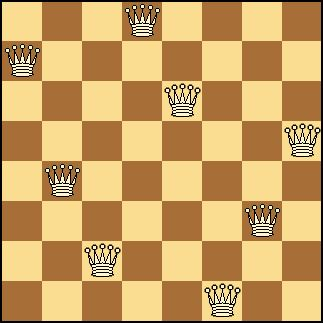
\includegraphics[]{huitreines.jpg}
\end{center}

\vspace{1em}

Ainsi nous avons 4 contraintes:

\begin{itemize}
    \item Il faut placer N Reines sur l'échiquier
    \item 2 Reines ne peuvent être sur la même ligne
    \item 2 Reines ne peuvent être sur la même colonne
    \item 2 Reines ne peuvent être sur toutes les diagonales de l'échiquier.
\end{itemize}

Il se trouve que nous pouvons transformer ces contraintes pour n'en garder que 3:

\begin{itemize}
    \item Il faut une et une seule reine sur chaque ligne
    \item Il faut une et une seule reine sur chaque colonne
    \item 2 Reines ne peuvent être sur toutes les diagonales de l'échiquier.
\end{itemize}

On note la variable $p_i^j$. On considère que cette variable est vraie si et seulement si il y a une reine sur la case sur i-ième ligne et sur la j-ième colonne.

On note la formule sous forme normale conjonctive $\phi_i$ la formule qui correspond au fait qu'une reine apparaît une seule et unique fois sur la i-ième ligne.

$$ \phi_i = \Big( \bigvee_{1 \leq j \leq N} p_i^j \Big) \land \Big( \underset{r \neq s}{\bigwedge_{1 \leq r, s \leq N}} \big( \lnot{p_i^r} \lor \lnot{p_i^s} \big) \Big) $$

La première partie de la conjonction désigne ici le fait qu'il y ait au moins une reine sur chaque ligne, et la seconde partie de la conjonction, désigne le fait qu'il ne peut y avoir plus d'une reine sur chaque ligne.

On note enfin $\psi_j$ la formule qui correspond à $\phi_i$ mais pour les colonnes. On construit la formule de la même façon en inversant l'indice du haut avec l'indice du bas. Ce qui donne :

$$ \psi_j = \Big( \bigvee_{1 \leq i \leq N} p_i^j \Big) \land \Big( \underset{r \neq s}{\bigwedge_{1 \leq r, s \leq N}} \big( \lnot{p_r^j} \lor \lnot{p_s^j} \big) \Big) $$

Il nous reste à représenter la dernière contrainte. On note $D$ l'ensemble des diagonales de l'échiquier. On peut calculer cet ensemble facilement en prenant les cases de la première ligne et de la première colonne par exemple puis en faisant une translation vectorielle jusqu'à sortir de l'échiquier. $D$ contient alors des ensembles de variables propositionnelles qui appartiennent à la même diagonale. On note alors la dernière contrainte par $\mu$:

$$ \mu = \bigwedge_{diag \in D} \Big( \underset{p \neq q}{\bigwedge_{p, q \in diag}} \big( \lnot{p} \lor \lnot{q} \big) \Big) $$

On peut ainsi représenter le problème des N Reines par :

$$ \Big( \bigwedge_{1 \leq i \leq N} \phi_i \Big) \land \Big( \bigwedge_{1 \leq j \leq N} \psi_j \Big) \land \mu $$

\subsection{Problème du sudoku}

Le Sudoku est un jeu qui consiste à remplir une grille de taille 9x9 contenant des blocs de taille 3x3 avec des chiffres allant de 1 à 9 telles que dans chaque bloc, sur chaque ligne et sur chaque colonne, chaque chiffre n'apparait qu'une seule et unique fois. Voici un grille partiellement remplie comme on peut trouver dans le commerce :

\begin{center}
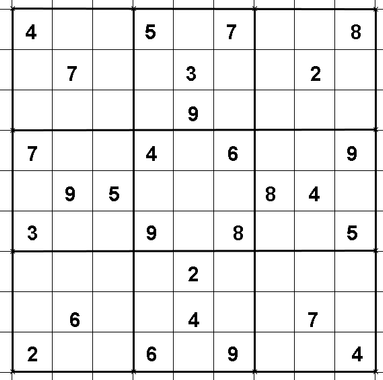
\includegraphics[scale=0.7]{sudoku.png}
\end{center}

Il a plusieurs contraintes à respecter lorsque l'on essaye de résoudre le problème :
\begin{itemize}
    \item Une case doit contenir exactement un chiffre.
    
    \item Tous les chiffres de 1 à 9 doivent être présents sur chaque ligne.
    \item Il ne peut y avoir plus deux fois le même chiffre sur la même ligne.

    \item Tous les chiffres de 1 à 9 doivent être présents sur chaque colonne.
    \item Il ne peut y avoir plus deux fois le même chiffre sur la même colonne.

    \item Tous les chiffres de 1 à 9 doivent être présents dans chaque bloc.
    \item Il ne peut y avoir plus deux fois le même chiffre dans le même bloc.
\end{itemize}

Pour tout $1 \leq n \leq 9$, $1 \leq i \leq 9$ et $1 \leq j \leq 9$, on considère $n_i^j$ la variable propositionnelle que l'on interprète par "Si $n_i^j$ est vraie alors il y a $n$ dans la case sur la i-ème ligne et sur la j-ème colonne". \\

On pose $\mu_i^j$ la formule qui modélise le fait que la case sur la i-ème ligne et la j-ème colonne contient exactement un chiffre.

$$\mu_i^j = \Big( \bigvee_{1 \leq n \leq 9} n_i^j \Big) \land \Big( \underset{m \neq m}{\bigwedge_{1 \leq n,m \leq 9}} \big( \lnot{n_i^j} \lor \lnot{m_i^j} \big) \Big)$$ 

La première partie correspond au fait qu'il y ait au moins un seul chiffre dans la case alors que la deuxième correspond au fait qu'il ne peut y avoir deux chiffres dans cette même case.\\
On note la formule sous forme normale conjonctive $\phi_i^n$ la formule qui correspond au fait que le chiffre $n$ est présent une seule et unique fois sur la i-ème ligne.

$$ \phi_i^n = \Big( \bigvee_{1 \leq j \leq 9} n_i^j \Big) \land \Big(\underset{r \neq s}{\bigwedge_{1 \leq r, s \leq 9}} \big( \lnot{n_i^r} \lor \lnot{n_i^s} \big) \Big) $$

Cette formule est construite de la même manière que la formule $\phi_i$ pour le problème des N reines.
On note $\Phi_i$ la formule correpondant au fait que tous les chiffres sont présents une seule et unique fois sur la i-ème ligne.

$$\Phi_i = \Big( \bigwedge_{1 \leq n \leq 9} \phi_i^n \Big)$$

On note $\psi_j^n$ la formule qui correspond à $\phi_j^n$ mais pour les colonnes. Il suffit, pour la construire, d'inverser i et j dans la formule.
On pose alors $\Psi_j$ la formule dont la signification est équivalente à celle de $\Phi_i$ mais pour les colonnes.

Enfin, il reste à modéliser les contraintes sur les blocs de la grille exactement de la même façon que pour les lignes et les colonnes. Ainsi, la formule $\Theta_b$ correspond au fait que chaque chiffre n'est présent qu'une seule et unique fois dans le bloc $b \in B$ (B étant  l'ensemble des blocs de la grille). \\
On peut alors représenter le problème de la grille de Sudoku vide ainsi :

$$\Big( \underset{1 \leq j \leq 9}{\bigwedge_{1 \leq i \leq 9}} \mu_i^j \Big) \land \Big( \bigwedge_{1 \leq i \leq 9} \Phi_i \Big) \land \Big( \bigwedge_{1 \leq j \leq 9} \Psi_j \Big) \land \Big( \bigwedge_{b \in B} \Theta_b \Big)$$

Pour modéliser le problème d'une grille partiellement remplie, il suffit de rajouter des clauses unitaires. Ainsi, pour toute case sur la i-ème ligne et la j-ème colonne contenant déjà $n$, on rajoute la clause qui ne contient que le littéral $n_i^j$ à la formule précédente. \\

Cette modélisation fonctionne pour toutes les formes de grille de Sudoku acceptables, c'est-à-dire que pour une grille $(n \times m) \times (n \times m)$, la taille des blocs doivent être $n \times m$.

\subsection{Problème des nonogrammes}

Un nonogramme (ou picross en anglais) consiste à remplir une grille de taille quelconque de cases noirs ou blanches afin de respecter certaines contraintes sur les lignes et sur les colonnes.

\vspace{2em}

\begin{center}
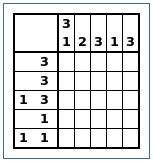
\includegraphics[]{nonogram1.png}
\end{center}

\vspace{2em}

Sur ce petit exemple, pour chaque ligne et colonne, il faut former des blocs continus de cases noirs.

Pour la première ligne, il faut former un seul bloc continu de 3 cases, soit sur les 3 premières cases, soit sur les 3 cases du milieu, soit sur les 3 dernières cases.

Pour la première colonne, il faut former deux blocs de cases noirs, le premier bloc contient 3 cases noirs et le second bloc ne contient qu'une seule case. 2 blocs ne peuvent se suivent car ils formeraient un seul bloc, ainsi sur la première colonne, il faut 3 cases noirs sur les 3 premières cases et une case noire sur la dernière case.

On peut donc poursuivre le raisonnement et obtenir une figure de cases noirs.

\vspace{2em}

\begin{center}
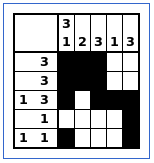
\includegraphics[]{nonogram1-solution.png}
\end{center}

\vspace{2em}

On peut évidemment imaginer des nonogrammes bien plus gros qui souvent sont beaucoup plus durs à résoudre par un être humain.

\vspace{2em}

\begin{center}
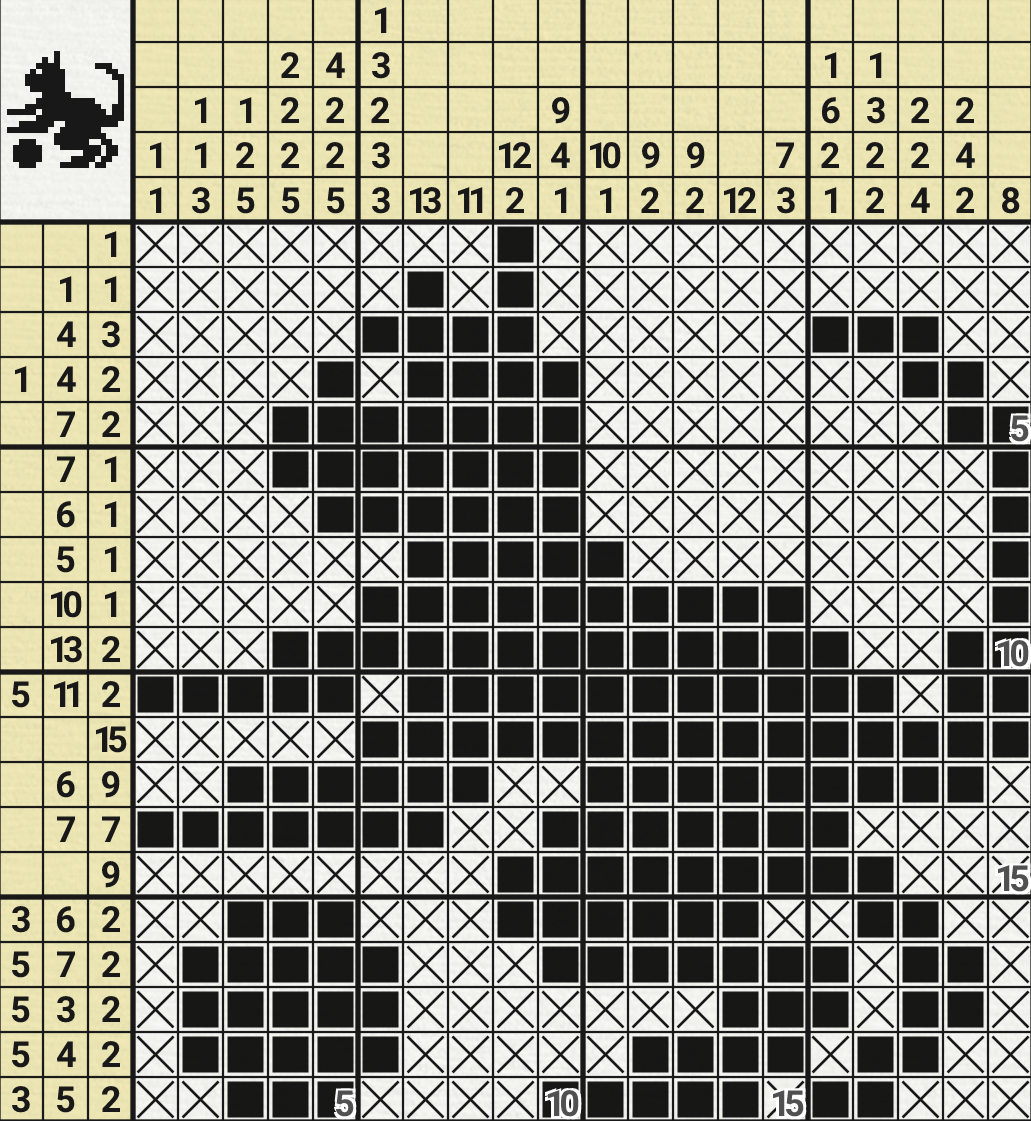
\includegraphics[width=.75\textwidth,height=.75\textwidth]{cat_picross.png}
\end{center}

\vspace{2em}

Nous allons maintenant représenter ce problème à l'aide de contraintes.

\begin{itemize}
    \item Un bloc doit être présent une seule et unique fois sur sa ligne / colonne
    \item Deux blocs ne doivent pas se chevaucher 
    %surpasser
    et doivent laisser au moins une case blanche d'écart.
    \item Toutes les cases d'un bloc sont de couleurs noirs
    \item Une case noire appartient à un bloc de sa colonne et un bloc de sa ligne.
\end{itemize}

Ces contraintes sont facilement représentables à l'aide de 4 formules que l'on peut transformer dans une formule FNC, que l'on pourra donner à un SAT-solveur et résoudre ainsi le nonogramme.

\newpage

\section*{Conclusion}

Nous avons montré dans ce document qu'il existe de nombreux moyens d'apporter une réponse à une instance du problème SAT.
%Toutes les solutions valables utilisent l'algorithme CDCL en utilisant des heuristiques différentes.
Actuellement, les meilleurs SAT-solveurs sont ceux basés sur l'algorithme CDCL mais utilisant des heuristiques différentes.
C'est notamment sur ce point et sur l'implémentation que les SAT-solveurs de compétition se départagent.

Cook est le premier à avoir trouvé un ensemble NP complet, à savoir SAT. Depuis on a obtenu également de nombreux autres problèmes NP-complets.
On peut nommer les 21 problèmes de Karp ainsi que certains problèmes NP-complets connus comme le problème du voyageur du commerce.

\nocite{*}

\bibliographystyle{plain}
\bibliography{bibli}

\end{document}
